\documentclass[a4paper,11pt]{jsarticle}
\usepackage{graphicx}
\usepackage{wrapfig}
\usepackage{amsmath,amssymb,amsthm}
\usepackage{amssymb}
\usepackage{ascmac}
\usepackage{subfigure}
\usepackage{bm}
\usepackage{setspace}
\usepackage{cases}%左かっこつけるときに必要だった
\usepackage{leftidx}%行列表示用?
\usepackage{fancyhdr}
\usepackage{graphicx}
\usepackage{float}
\usepackage{booktabs}
\usepackage{url}
\usepackage{bm}
\usepackage{verbatim}
\usepackage{calc} 

\setlength{\headsep}{5mm}
\setlength{\oddsidemargin}{-0.5zw} %→にズラす
\setlength{\textheight}{37\baselineskip}
\addtolength{\textheight}{\topskip}
\setlength{\topmargin}{-10mm}
\setlength{\textwidth}{45zw} %文章の幅
\setlength{\textheight}{215mm}
\setlength{\parindent}{1zw}%箇条書きの一文字下げ
\pagestyle{fancy}

\newtheorem{theorem}{定理}
\newtheorem{prop}[theorem]{命題}
\newtheorem{lemma}[theorem]{補題}
\newtheorem{cor}[theorem]{系}
\newtheorem{example}[theorem]{例}
\newtheorem{definition}[theorem]{定義}
\newtheorem{rem}[theorem]{注意}
\newtheorem{guide}[theorem]{参考}
\renewcommand{\proofname}{証明}

\numberwithin{theorem}{section}  % 定理番号を「定理2.3」のように印刷
\numberwithin{equation}{section} % 式番号を「(3.5)」のように印刷
\newcommand{\argmax}{\mathop{\rm arg~max\,}\limits}
\newcommand{\argmin}{\mathop{\rm arg~min\,}\limits}
\newcommand{\st}{\mathop{\rm subject~to\,}\limits}
\newcommand{\sign}{\mathop{\rm sign\,}\limits}

\newcommand{\dom}{\mathop{\mathrm{\bf dom}}\nolimits}
\newcommand{\minimize}{\mathop{\mathrm{\rm minimize}}\limits}
\newcommand{\maximize}{\mathop{\mathrm{\rm maximize}}\limits}

\lhead{2012年度・CG第1回レポート}
\chead{}
\rhead{12M42340}
\lfoot{チョウ シホウ}
\cfoot{\thepage}
\rfoot{6月11日}
\renewcommand{\footrulewidth}{0.4pt}
\title{2012年度・CG第1回レポート}
\author{12M42340 チョウ シホウ}
\date{7月2日}


\begin{document}
\pagenumbering{roman}
%\tableofcontents
%\cleardoublepage
\pagenumbering{arabic}
\renewcommand{\thepart}{\arabic{part}}

%\thispagestyle{empty}

\begin{itembox}[l]{問題1}
The Fourier transform of the image whose density $g$ is defined by
\[g(x, y) = \sin(ax + b \sin(cy))\],
where a, b, and c are constants, gives a set of impulse functions. Derive the impulse functions, and illustrate them in frequency domain.
\end{itembox}
\begin{figure}[H]
\includegraphics[bb=0 0 444 451,width=10cm]{img1.pdf}
\end{figure}
\newpage
\begin{itembox}[l]{問題2}
In the following two graphs, a red point represents a delta function, and these graphs correspond to a sinusoid wave in image domain. Derive the sinusoid wave by 2 dimensional Inverse Fourier Transform.
\end{itembox}
\begin{figure}[H]
\includegraphics[bb=0 0 250 260]{img2.png}
\end{figure}
\newpage
\begin{itembox}[l]{問題3}
Illustrate this transformation on the next coordinate system graph, just like the illustration of the HSV color coordinate system in a handout of this lecture.
\end{itembox}
HSLの定義により,
\begin{eqnarray*}
L &=& \frac{1}{2}(\max+\min) \\
S &=& \begin{cases}
0 & \text{if} L = 0 \text{if} \max = \min\\
\frac{\max-\min}{\max+\min} & \text{if} 0<L\le\frac{1}{2}\\
\frac{\max-\min}{2-\max-\min} & \text{if} L\ge \frac{1}{2}
\end{cases}
\end{eqnarray*}
$H$はHSVの定義と同じく,色相の回旋角度を表す.$L$は最大値と最小値の平均を取り,$L$の値が$\frac{1}{2}$以上かどうかによって$S$を決めるため,次は$L$の値によって別々示す.

\begin{figure}[H]
\includegraphics[width=12cm]{p3_1a.ps}
\caption{$L<\frac{1}{2}$}
\end{figure}
\begin{figure}[H]
\includegraphics[width=12cm]{p3_1b.ps}
\caption{$L<\frac{1}{2}$}
\end{figure}
\begin{figure}[H]
\includegraphics[width=12cm]{p3_2a.ps}
\caption{$L<\frac{1}{2}$}
\end{figure}
\begin{figure}[H]
\includegraphics[width=12cm]{p3_2b.ps}
\caption{$L<\frac{1}{2}$}
\end{figure}

\newpage
\begin{itembox}[l]{問題4}
\begin{enumerate}
\item
Calculate the point for each pigment illuminated by a D65 light source on CIEXYZ 2degree. Here, assume that the values at less than 400nm are equal to the value at 400nm and the values at greater than 700nm are equal to the value at 700nm, and approximate the spectrum of the D65 light by black-body radiation at 6504K.
\item
Plot them and draw a triangle of sRGB color space on the same xy color diagram.
\item
Mark pigments which cannot be displayed correctly on sRGB monitors.
\item
Think of a method to display such colors on sRGB monitors as natural as possible and explain it. The explanation has to mention problems by the method.
\end{enumerate}
\end{itembox}
\begin{enumerate}
\item

次の\textbf{Color Matching Function}を用いて各Pigmentの\textbf{Reflect Function}に対応するXYZ値を算出する.
\begin{eqnarray*}
\mathcal{X} = k\int_{400}^{700} D_{65}(\lambda)x(\lambda)r_{\text{plot}}(\lambda) d \lambda \\
\mathcal{Y} = k\int_{400}^{700} D_{65}(\lambda)y(\lambda)r_{\text{plot}}(\lambda) d \lambda \\
\mathcal{Z} = k\int_{400}^{700} D_{65}(\lambda)z(\lambda)r_{\text{plot}}(\lambda) d \lambda \\
\end{eqnarray*}
\begin{equation*}
X = \frac{\mathcal{X}}{\mathcal{X} + \mathcal{Y} + \mathcal{Z}}\,\,\,
Y = \frac{\mathcal{Y}}{\mathcal{X} + \mathcal{Y} + \mathcal{Z}}\,\,\,
Z = \frac{\mathcal{Z}}{\mathcal{X} + \mathcal{Y} + \mathcal{Z}}
\end{equation*}
但し
\begin{itemize}
\item $\lambda$:波長
\item $D_{65}(\lambda)$:光源データ\\
\,\,\,\,\,\,\,\,\,\,\,\,\,\,\,\,\,\,\,\,\,\,\,\,\url{http://cvrl.ioo.ucl.ac.uk/database/data/cie/Illuminantd65.csv}
\item $x(\lambda),y(\lambda),z(\lambda)$:\textbf{XYZ\_CIE\_2.dat}に測定されたデータ
\item $r_{\text{plot}}$:各plotの\textbf{Pigments File}に定義された反射関数.
\end{itemize}
\begin{table}[H]
\caption{各Plotに対応するXYZ値}
\begin{center}
\begin{tabular}{lccc}
\toprule
Plot & $X$ & $Y$ & $Z$  \\
\midrule
1 & $0.556680$ & $0.349468$ & $0.093852$\\
6 & $0.540825$ & $0.326594$ & $0.132581$\\
15 & $0.500518$ & $0.251735$ & $0.247748$\\
33 & $0.312706$ & $0.329460$ & $0.357834$\\
41 & $0.321685$ & $0.340942$ & $0.337373$\\
46 & $0.317175$ & $0.334973$ & $0.347852$\\
51 & $0.172133$ & $0.119266$ & $0.708601$\\
58 & $0.198234$ & $0.197832$ & $0.603933$\\
64 & $0.294274$ & $0.226222$ & $0.479504$\\
72 & $0.229489$ & $0.404458$ & $0.366053$\\
74 & $0.261645$ & $0.430408$ & $0.307948$\\
84 & $0.503193$ & $0.450467$ & $0.046340$\\
92 & $0.456986$ & $0.485291$ & $0.057723$\\
\bottomrule
\end{tabular}
\end{center}

\end{table}

\item Wikipediaにより,sRGB色空間に於けるRed,Green,BuleとWhiteはそれぞれ次である.
\begin{table}[H]
\caption{The sRGB gamut}
\begin{center}
\begin{tabular}{|c|c|c|c|c|}
\hline
Chromaticity & Red & Green & Blue & White point \\
\hline
$X$& 	$0.6400$& 	$0.3000$& 	$0.1500$& 	$0.3127$\\
$Y$& 	$0.3300$& 	$0.6000$& 	$0.0600$& 	$0.3290$\\
$Z$& 	$0.0300$& 	$0.1000$& 	$0.7900$& 	$0.3583$\\
\hline
\end{tabular}
\end{center}
\label{default}
\end{table}
$XY$空間に描くと,次の三角形になる.「○」印の点は各Pigmentsである.
\begin{figure}[H]
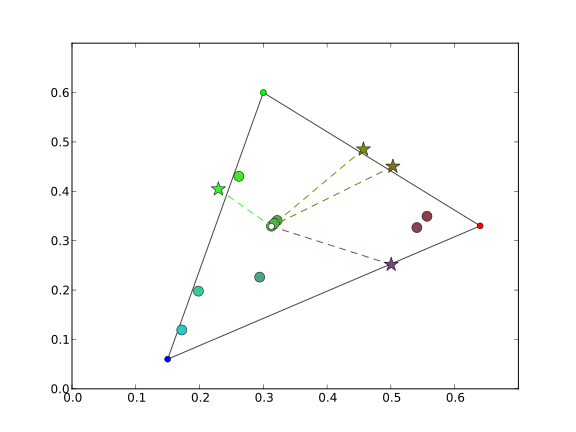
\includegraphics[width=14.5cm]{chrome.ps}
\caption{sRBG色空間}
\label{CHROME}
\end{figure}
\item 図\ref{CHROME}に於ける「★」印の点はsRGB空間に入られない点である.
\item sRGB空間で表示できない点をsRGB空間の中の近い色の点を用いてシミュレートすれば良い.図\ref{CHROME}の破線のように,白点(White Point)からsRGB Gamutに含まれない点に線を引き,その線とsRGB Gamutの交点の色を使うとsRGB以外の点も表示できる.
\end{enumerate}

\end{document}